
  \textit{Arrowized FRP} (AFRP
\cite{nilsson2002:arrows} \cite{hudak2002:arrows}) intenta
resolver los problemas de la FRP Clásica cambiando la forma
en la que se crean los programas.
  En éste paradigma, tampoco se toman en cuenta por separado los
eventos, se utiliza la misma definición de señal que en RT-FRP.

\begin{definicion}
  Señal (Signal).
  \center{
    $\textbf{Signal}\ \alpha = \textbf{Time} \rightarrow \alpha$
  }
\end{definicion}

  En lugar de permitir que se manipulen las señales como valores
de primera clase, ésto se prohibe y se define el concepto de
\textit{Signal Functions} (funciones sobre señales). El programador
tendrá acceso sólo a las señales utilizándolas.

\begin{definicion}
  Funciones sobre señales (Signal Functions).
  \center{
    $\textbf{SF}\ \alpha\ \beta = \textbf{Signal}\ \alpha \rightarrow \textbf{Signal}\ \beta$
  }
\end{definicion}

  Sin embargo, la representación de \texttt{SF} no es accesible al
desarrollador, en lugar de eso se define un conjunto de funciones
sobre señales primitivas y un conjunto de combinadores
 para componerlas.

\begin{figure}[h]
\begin{center}
  \caption{Combinadores. (Imagen tomada de \cite{yampa})}
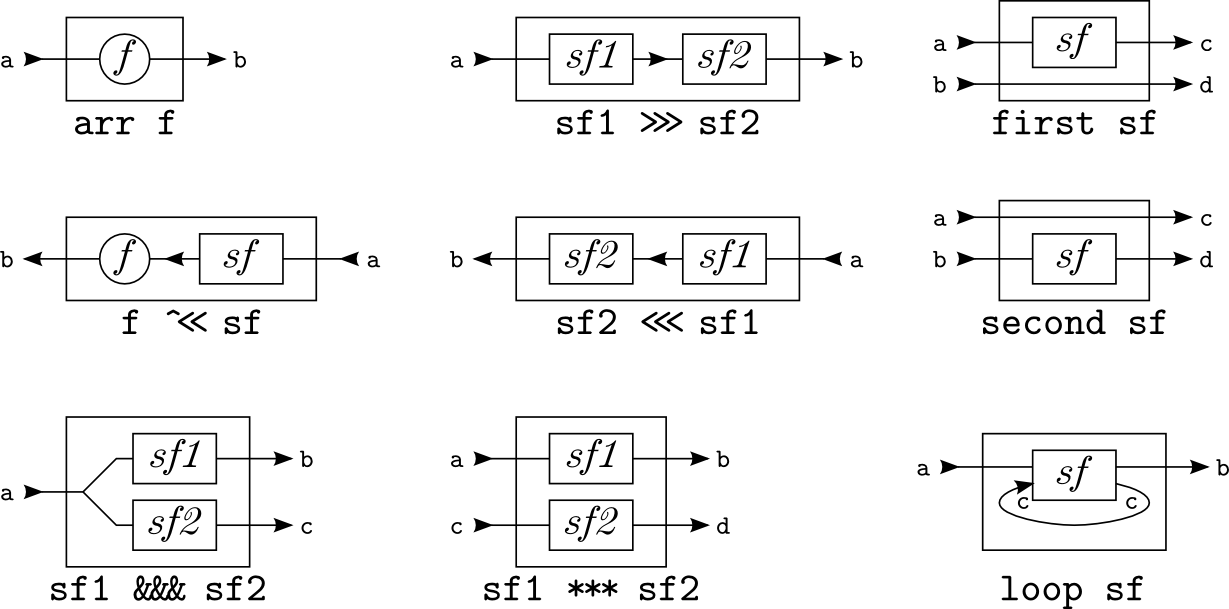
\includegraphics[width=0.9\textwidth]{graphs/yampasf.png}
\label{fig:arrowcombinators}
\end{center}
\end{figure}

  AFRP está basado en \textit{Arrows} \cite{hughes1998:arrows}
una generalización del concepto de \textit{Monads}. En particular
\texttt{SF} es una instancia de la clase \textit{Arrow}.

  Un programa es una \texttt{SF} global, compuesta por un conjunto
de otras \textit{Signal functions}, y un intérprete corre ésta instancia
global.

  En la Figura \ref{fig:arrowcombinators} se puede ver un conjunto
extenso de combinadores, sin embargo se
puede definir un conjunto minimal utilizando sólo
los combinadores \texttt{arr},
$\gg$ y \texttt{first}, aunque no es el único.

  \paragraph{Yampa}
  El framework \textit{Yampa} \cite{yampa} embebido en Haskell, 
define los operadores de la Figura \ref{fig:arrowcombinators}
para combinar señales y aplicar funciones sobre ellas.



%TODO(Marcos): Ejemplos de los operadores y su uso?

